\clearpage

\lehead[]{\sf\hspace*{-2.00cm}\textcolor{white}{\colorbox{lightblue}{\parbox[c][0.70cm][b]{1.60cm}{
\makebox[1.60cm][r]{\thechapter}\\ \makebox[1.60cm][r]{ÜBUNG}}}}\hspace{0.17cm}\textcolor{lightblue}{\chaptertitle}}
\rohead[]{\textcolor{lightblue}{\chaptertitle}\sf\hspace*{0.17cm}\textcolor{white}{\colorbox{lightblue}{\parbox[c][0.70cm][b]{1.60cm}{\thechapter\\
ÜBUNG}}}\hspace{-2.00cm}}
%\chead[]{}
\rehead[]{\textcolor{lightblue}{AvHG, Inf, My}}
\lohead[]{\textcolor{lightblue}{AvHG, Inf, My}}

\section{Fehlerbehandlung -- Übungen}

\subsection{Aufgabe 1: Währungsrechner}

Schreibe ein Programm, das zwischen zwei Währungen umrechnen kann (zum Beispiel
zwischen Euro und Britischen Pfund). Damit das Programm nicht veraltet, wird der
aktuelle Währungskurs in einem \myClass{JTextField} eingegeben. Die Oberfläche
könnte z.B. so aussehen:

\begin{center}
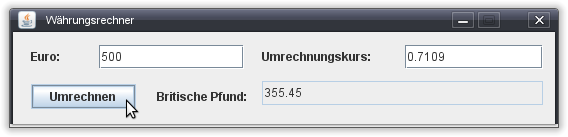
\includegraphics[width=0.9\textwidth]{./inf/SEKII/25_Java_Exceptions/Waehrungsrechner.png}
\end{center}

Das Ausgabe-Textfeld soll nicht editierbar sein. Programmiere zunächst die
Oberfläche (ohne Umrechnungsfunktionalität) und gehe dann in folgenden
Teilschritten vor:

\begin{compactenum}[a)]
\item Leite drei verschiedene Exception-Klassen von der Superklasse
\myClass{Exception} ab. Alle Exception-Klassen sollen einen parameterlosen
Konstruktor besitzen, der automatisch den in Klammern angegebenen Fehlertext generiert:

\begin{compactitem}
\item \myClass{LeerException}  (\glqq Sie haben die Eingabe in das Textfeld
vergessen. Das Textfeld ist leer.\grqq ) 
\item \myClass{KommaException} (\glqq Sie haben in der Fließkommazahl ein Komma
an Stelle eines Punktes eingegeben.\grqq )
\item \myClass{ZeichenException} (\glqq Sie haben ein unerlaubtes Zeichen
eingegeben.
Zulässig sind nur Ziffern und ein Punkt.\grqq )
\end{compactitem}

\item Schreibe eine Methode \lstinline|zahlAuslesen()|, der ein Textfeld als
Parameter übergeben wird. Die Methode überprüft die Eingabe im Textfeld auf
Korrektheit und wirft bei Eingabefehlern des Benutzer die  entsprechende
Exception. Wenn der Benutzer den Text korrekt eingegeben hat, konvertiert sie
den Text mit der Methode \lstinline|Double.parseDouble()| in einen
\lstinline|double|-Wert und gibt die so erzeugte Zahl als Rückgabewert zurück.

\item Programmiere den Code zur Währungsumrechnung unter Verwendung der
Methode \lstinline|zahlAuslesen()|. Fange eventuell auftretende Exceptions ab
und gib den Fehlertext (inklusive des Namens der Fehlerklasse) in einer
Message-Box aus.
\end{compactenum}


\subsection{Aufgabe 2: Benzinkosten berechnen}

Schreibe ein Programm, das die Benzinkosten für eine bestimmte Strecke (zum
Beispiel Bremen -- Hamburg) berechnet. Der Benutzer soll folgende Eingaben
vornehmen können:

\begin{compactitem}
\item die Strecke in km 
\item der Verbrauch des PKWs pro 100 km 
\item der aktuelle Benzinpreis (in Euro/Liter)
\end{compactitem}

Im Hauptfenster gibt es drei Textfelder zu Eingabe der Werte und einen Button,
mit dem die Berechnung gestartet wird. Die vom Benutzer eingegebenen Strings
müssen zur Berechnung mit der Methode \lstinline|Double.parseDouble()| in
Fließkommazahlen umgewandelt werden. Falls der Benutzer eine fehlerhafte
Eingabe gemacht hat, wirft die Methode \lstinline|parseDouble()| eine
\myClass{NumberFormatException}. Fange diese Exception in einem
\lstinline|catch|-Block ab, und gib dem Benutzer gegebenenfalls eine für ihn
verständliche Fehlermeldung aus. (Eigene Exceptions brauchen bei dieser Übung
nicht generiert werden).

\begin{minipage}{0.5\textwidth}
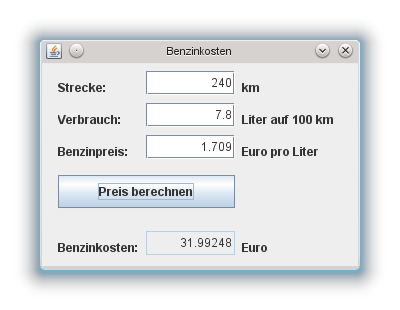
\includegraphics[width=1.0\textwidth]{./inf/SEKII/25_Java_Exceptions/Benzinkosten.png}
\end{minipage}
\hfill
\begin{minipage}{0.5\textwidth}
\subsubsection{Konvertierung von \myClass{String} in \myClass{double}}

Beispiel:

\begin{lstlisting}
String text = "3.14";
double pi = Double.parseDouble(text);
\end{lstlisting}
\end{minipage}


\subsection{Aufgabe 3: Andere Programme starten}

Mit Hilfe der Klasse \myClass{Runtime} können von einem Java-Programm aus andere
Programme gestartet werden. Ein Objekt der Klasse \myClass{Runtime} holt man
sich mit einer statischen Methode von der Klasse \myClass{Runtime} selbst:

\begin{lstlisting}
public static Runtime getRuntime()
\end{lstlisting}

Anschließend kann man mit der folgenden Methode der Klasse \myClass{Runtime} ein
anderes Programm starten:

\begin{lstlisting}
public Process exec(String command) throws IOException
\end{lstlisting}

Die Methode wirft eine \myClass{IOException}, wenn das Programm nicht gefunden
werden konnte.

Als Rückgabewert erhält man ein Objekt der Klasse \myClass{Process} (Anmerkung:
Prozess ist das Fachwort für ein laufendes Programm.). Mit Hilfe dieses
Objektes kann man mit dem gestarteten Programm \glqq kommunizieren\grqq , in dem
man zum Beispiel die folgenden Methoden der Klasse \myClass{Process} aufruft:

\begin{lstlisting}
public void destroy()
\end{lstlisting}

Mit Hilfe dieser Methode wird das laufende Programm auf harte Weise (ohne
Benutzerabfrage) beendet.

\begin{lstlisting}
public int waitFor() throws InterruptedException
\end{lstlisting}

Mit der Methode \lstinline|waitFor()| kann man im aktuellen Programm auf die
Beendigung des gestarteten Programms warten. Dies ist zum Beispiel sinnvoll,
wenn das fremde Programm wichtige Daten berechnet, die zur weiteren Arbeit
benötigt werden. Das aktuelle Programm läuft nicht mehr weiter,  bis das fremde
Programm beendet wurde. Als Rückgabewert erhält man die Zahl, die das fremde
Programm im \lstinline|exit()|-Aufruf zurückgibt. Dies ist normalerweise der
Wert 0, der für \glqq erfolgreich beendet\grqq\ steht. Die
\myClass{InterruptedException} kann nur theoretisch auftreten und darf ignoriert
werden. Man braucht jedoch einen Exception-Handler ohne Funktionalität, um den
Code durch den Compiler zu bekommen.

\subsubsection{Übungsaufgabe}

\begin{center}
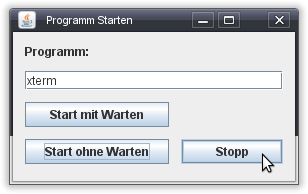
\includegraphics[width=0.4\textwidth]{./inf/SEKII/25_Java_Exceptions/ProgrammStart.png}
\end{center}

Erzeuge ein Programm mit der oben abgebildeten Oberfläche. Wenn man auf den
Button \glqq Start mit Warten\grqq\ drückt, wird das vom Benutzer angegebene
Programm gestartet und anschließend mit \lstinline|waitFor()| auf seine
Beendigung gewartet. Nach der Rückkehr des Aufrufs von \lstinline|waitFor()|
wird eine Meldung ausgegeben, in der der Rückgabewert des fremden Programms
mitgeteilt wird. Falls das Programm nicht gestartet werden kann, wird in einem
Exception-Handler eine entsprechende Fehlermeldung ausgegeben.

Wenn man auf den Button \glqq Start ohne Warten\grqq\ drückt, wird das Programm
einfach nur gestartet. Das zurückgegebene \myClass{Process}-Objekt wird in einer
globalen Variablen gespeichert. Wenn man auf den Stop-Button drückt, wird das
Programm, das in der \myClass{Process}-Variablen abgespeichert wurde, mit
\lstinline|destroy()| beendet. Falls in der \myClass{Process}-Variablen kein
fremdes Programm abgespeichert ist, gibt es eine \myClass{NullPointerException}.
Fange diese Exception mit einem Exception-Handler ab und gib gegebenenfalls
eine geeignete Fehlermeldung aus.
